\capitulo{5}{Resultados}
\label{cap:resultados}

\section{Evaluación comparativa de modelos}
\label{sec:evaluacion_modelos}

\subsection{Evaluación detallada y métricas clave}

Como primer paso para seleccionar el modelo más adecuado, se entrenaron cinco algoritmos de clasificación multiclase utilizando los datos originales del conjunto de entrenamiento, sin aplicar técnicas de balanceo ni ajuste de hiperparámetros. El objetivo de esta fase inicial fue obtener una visión general del rendimiento de cada modelo en condiciones estándar y valorar su comportamiento en un contexto clínico realista.

Los modelos evaluados fueron:

\begin{itemize}
    \item Regresión Logística
    \item Árbol de Decisión
    \item Máquina de Vectores Soporte (SVM)
    \item Random Forest
    \item Perceptrón Multicapa (MLP)
\end{itemize}

Cada modelo fue entrenado con validación cruzada estratificada (k=5), y se calcularon métricas fundamentales como \textbf{accuracy}, \textbf{F1-score macro}, \textbf{recall} por clase y \textbf{precisión} en la clase \texttt{Sleep Apnea}, de especial relevancia clínica.

En la Tabla~\ref{tab:comparativa-inicial} se muestran los resultados obtenidos por cada modelo en esta primera evaluación en condiciones estándar:

\begin{table}[H]
\centering
\small 
\begin{tabular}{lccccc}
\toprule
\textbf{Modelo} & \textbf{Accuracy} & \textbf{F1 Macro} & \textbf{Recall Ins.} & \textbf{Recall Apn.} & \textbf{Prec. Apn.} \\
\midrule
Random Forest       & 0.95 & 0.92 & 0.87 & 0.94 & 0.88 \\
MLP                 & 0.92 & 0.88 & 0.87 & 0.81 & 0.81 \\
Logistic Regression & 0.93 & 0.91 & 0.87 & 0.94 & 0.83 \\
Decision Tree       & 0.92 & 0.89 & 0.93 & 0.81 & 0.87 \\
SVM                 & 0.92 & 0.91 & 0.87 & 0.88 & 0.88 \\
\bottomrule
\end{tabular}
\caption{Rendimiento comparativo de los modelos en condiciones iniciales (sin ajuste ni balanceo).}
\label{tab:comparativa-inicial}
\end{table}

Para profundizar en la evaluación individual de los modelos, en las Figuras~\ref{fig:confusion_logreg} y~\ref{fig:metricas_logreg} se presentan los resultados iniciales del modelo \textit{Logistic Regression}, incluyendo su matriz de confusión y un resumen de métricas cuantitativas obtenidas con \texttt{classification\_report}. Este modelo se ha seleccionado como ejemplo representativo por su equilibrio entre rendimiento global e interpretabilidad, y se utiliza aquí para ilustrar el proceso de evaluación antes de aplicar técnicas de mejora.


\begin{figure}[H]
    \centering
    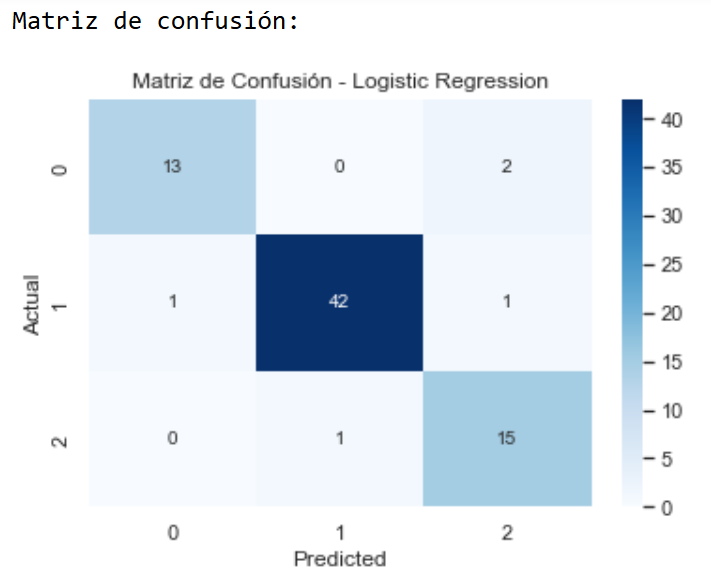
\includegraphics[width=0.6\linewidth]{img/matriz_confusion_logreg.png}
    \caption{Matriz de confusión del modelo \textit{Logistic Regression} sobre el conjunto de test.}
    \label{fig:confusion_logreg}
\end{figure}

\begin{figure}[H]
    \centering
    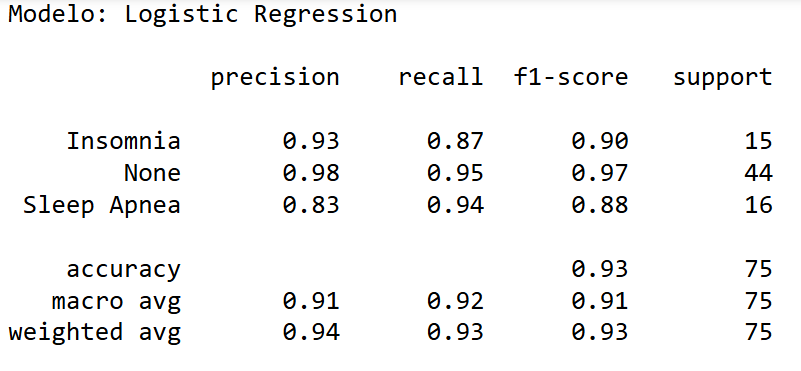
\includegraphics[width=0.65\linewidth]{img/metricas_logreg.png}
    \caption{Resumen de métricas del modelo \textit{Logistic Regression} generadas con \texttt{classification\_report} de \texttt{scikit-learn}.}
    \label{fig:metricas_logreg}
\end{figure}

Tal como se aprecia en la Tabla~\ref{tab:comparativa-inicial}, los modelos \textit{Random Forest} y \textit{Logistic Regression} destacan por sus elevados valores de \textit{accuracy} (0.95 y 0.93 respectivamente) y \textit{F1-score macro} (0.92 y 0.91), manteniendo además un rendimiento sólido en las clases patológicas. En particular, ambos modelos presentan un \textit{recall} en la clase \texttt{Sleep Apnea} de 0.94, lo que resulta clínicamente relevante. En cambio, el modelo \textit{MLP}, muestra menor sensibilidad en dicha clase (0.81), lo cual podría limitar su utilidad como herramienta de cribado inicial. 

Estos resultados iniciales constituyeron la base para aplicar estrategias de mejora, comenzando por el balanceo de clases mediante la técnica SMOTE, cuyo impacto se analiza a continuación.

\subsection{Impacto del balanceo con SMOTE}

Con el fin de analizar el impacto del desbalance de clases, se comparó el rendimiento de cinco modelos entrenados sobre los datos originales y sobre un conjunto equilibrado mediante la técnica \textbf{SMOTE} (Synthetic Minority Over-sampling Technique). Esta técnica genera nuevas muestras sintéticas para las clases minoritarias a partir de sus vecinos más cercanos, con el objetivo de mitigar los sesgos introducidos por el desequilibrio de clases.

Se entrenaron cinco modelos de clasificación bajo ambas condiciones: Regresión Logística, Árbol de Decisión, Máquina de Vectores Soporte (SVM), Random Forest y Perceptrón Multicapa (MLP).


Para cada modelo se calcularon métricas como \textit{accuracy}, \textit{F1-score macro} y \textit{recall} en la clase \texttt{Sleep Apnea}, considerada de mayor relevancia clínica. En la Tabla~\ref{tab:smote_comparacion} se muestra un resumen de estas métricas para facilitar la comparación inicial entre modelos con y sin SMOTE:


\begin{table}[H]
\centering
\resizebox{\textwidth}{!}{%
\begin{tabular}{|l|c|c|c|c|c|c|}
\hline
\rowcolor[HTML]{DAE8FC}
\textbf{Modelo} & \textbf{Accuracy (SMOTE)} & \textbf{Accuracy (No SMOTE)} & \textbf{F1 Macro (SMOTE)} & \textbf{F1 Macro (No SMOTE)} & \textbf{Recall Apnea (SMOTE)} & \textbf{Recall Apnea (No SMOTE)} \\
\hline
Logistic Regression & 0.93 & 0.93 & 0.92 & 0.91 & 1.00 & 0.94 \\
Decision Tree       & 0.93 & 0.91 & 0.91 & 0.87 & 0.94 & 0.81 \\
SVM                 & 0.92 & 0.92 & 0.90 & 0.91 & 1.00 & 0.88 \\
MLP                 & 0.92 & 0.92 & 0.89 & 0.88 & 0.81 & 0.81 \\
Random Forest       & 0.93 & 0.95 & 0.90 & 0.92 & 0.81 & 0.94 \\
\hline
\end{tabular}
}
\caption{Comparación resumida de rendimiento con y sin SMOTE.}
\label{tab:smote_comparacion}
\end{table}

A modo ilustrativo, se muestran a continuación las métricas detalladas y matrices de confusión del modelo \textit{Logistic Regression}, en ambos escenarios:

\begin{figure}[H]
    \centering
    \begin{minipage}{0.48\linewidth}
        \centering
        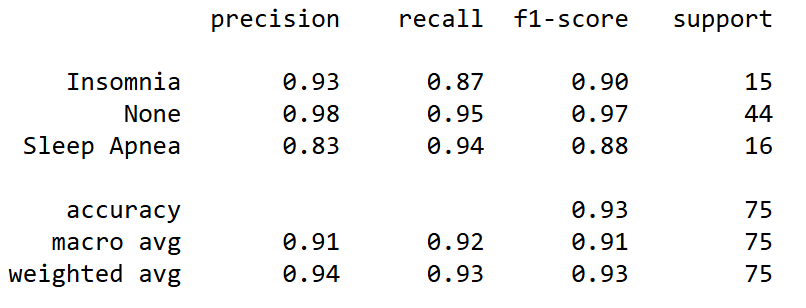
\includegraphics[width=\linewidth]{img/tablaLRsinSmote.png}
        \caption{Métricas del modelo \textit{Logistic Regression} sin SMOTE.}
        \label{fig:tabla_lr_sin_smote}
    \end{minipage}
    \hfill
    \begin{minipage}{0.48\linewidth}
        \centering
        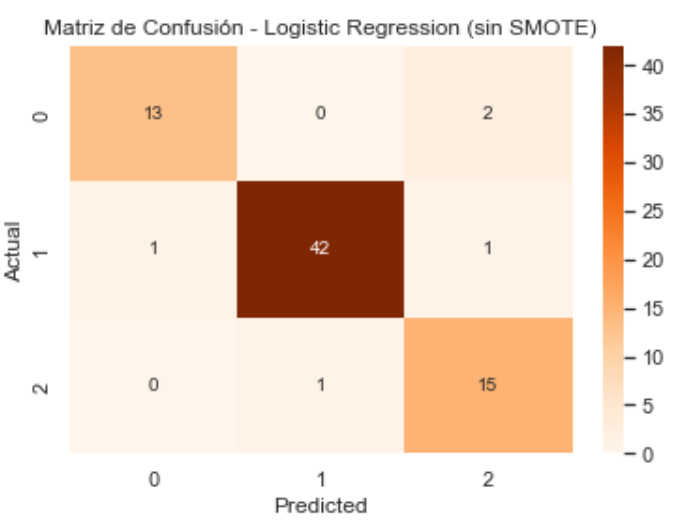
\includegraphics[width=\linewidth]{img/matrizLRsinSmote.png}
        \caption{Matriz de confusión del modelo \textit{Logistic Regression} sin SMOTE.}
        \label{fig:matriz_lr_sin_smote}
    \end{minipage}
\end{figure}

\begin{figure}[H]
    \centering
    \begin{minipage}{0.48\linewidth}
        \centering
        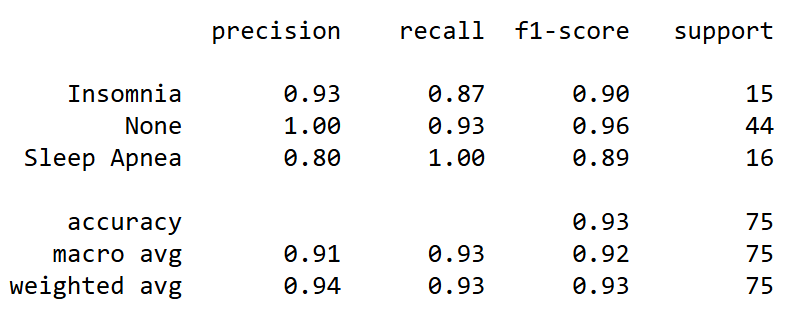
\includegraphics[width=\linewidth]{img/tablaLRsmote.png}
        \caption{Métricas del modelo \textit{Logistic Regression} con SMOTE.}
        \label{fig:tabla_lr_smote}
    \end{minipage}
    \hfill
    \begin{minipage}{0.48\linewidth}
        \centering
        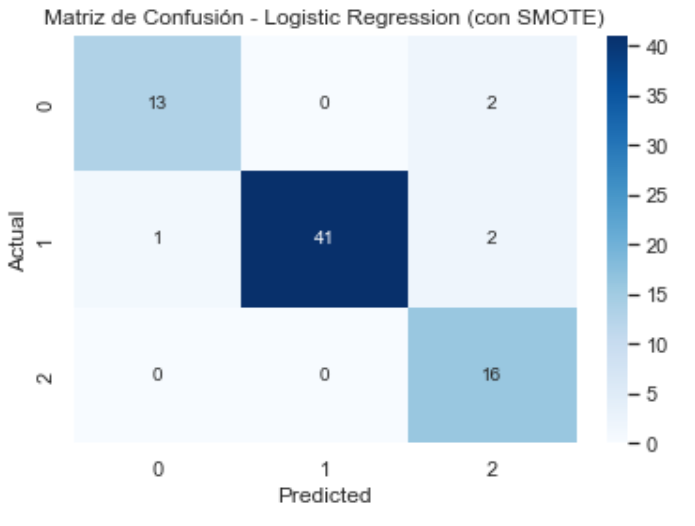
\includegraphics[width=\linewidth]{img/matrizLRsmote.png}
        \caption{Matriz de confusión del modelo \textit{Logistic Regression} con SMOTE.}
        \label{fig:matriz_lr_smote}
    \end{minipage}
\end{figure}

Además, la Figura~\ref{fig:comparativa_smote} muestra un análisis completo con todas las métricas evaluadas para los cinco modelos:

\begin{figure}[H]
    \centering
    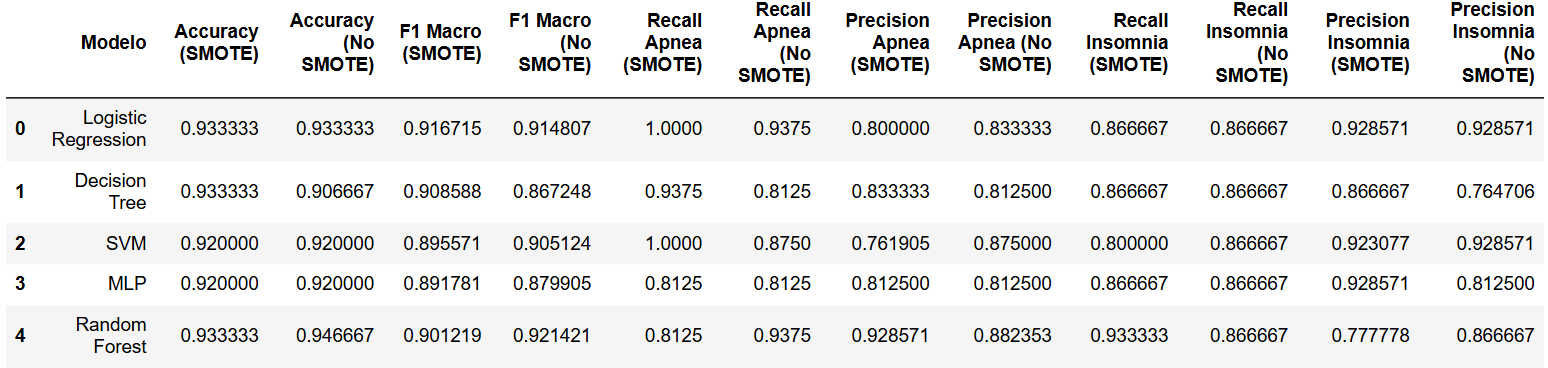
\includegraphics[width=1\linewidth]{img/comparativa_smote.png}
    \caption{Comparación de métricas clave con y sin SMOTE en los cinco modelos.}
    \label{fig:comparativa_smote}
\end{figure}


Los resultados mostraron que SMOTE mejora sistemáticamente el \textit{recall} de la clase \textit{Sleep Apnea} en la mayoría de modelos, lo cual es clínicamente positivo al tratarse de una clase minoritaria. Sin embargo, este aumento suele ir acompañado de una ligera caída en la \textit{precisión}, lo que sugiere un mayor número de falsos positivos.

En el caso de \textit{Logistic Regression}, por ejemplo, el \textit{recall} de \texttt{Sleep Apnea} pasó de 0.94 a 1.00 con SMOTE, pero su precisión cayó del 0.83 al 0.80. En modelos como \textit{Decision Tree}, el \textit{recall} también aumentó significativamente (0.81 → 0.94), aunque sin mejoras globales contundentes. Por el contrario, en el modelo \textit{MLP}, SMOTE no aportó mejoras relevantes, manteniendo el mismo \textit{recall} (0.81) y reduciendo ligeramente la precisión.

En el caso de \textit{Random Forest}, aplicar SMOTE redujo inesperadamente el \textit{recall} de \textit{Sleep Apnea} (de 0.94 a 0.81), indicando una posible pérdida de sensibilidad tras el sobremuestreo.


Dado que el impacto de SMOTE fue inconsistente entre modelos, y considerando el riesgo de sobreajuste en ciertos casos, se optó por no incluir esta técnica en la versión final del sistema. En su lugar, se utilizó la opción \texttt{class\_weight='balanced'} junto con calibración probabilística posterior, lo que permitió mantener un buen rendimiento sin comprometer la estabilidad del modelo.


\subsection{Ajuste de hiperparámetros y calibración}

Con el objetivo de mejorar el rendimiento predictivo de cada modelo, se realizó un proceso de búsqueda de hiperparámetros empleando las funciones \texttt{GridSearchCV} o \texttt{RandomizedSearchCV}, en función del tamaño del espacio de búsqueda y del coste computacional. Esta optimización se llevó a cabo sobre el conjunto de entrenamiento utilizando validación cruzada estratificada con \texttt{cv=5}.

Según el tipo de modelo, se definió como métrica objetivo el \texttt{accuracy} o, en modelos más sensibles al desbalance, el \texttt{F1-score macro}, priorizando así un compromiso entre precisión y sensibilidad global. En la Tabla~\ref{tab:hiperparametros_optimos} se resumen los mejores hiperparámetros encontrados para cada algoritmo:

\begin{table}[H]
\centering
\resizebox{\textwidth}{!}{%
\begin{tabular}{|l|l|}
\hline
\rowcolor[HTML]{DAE8FC}
\textbf{Modelo} & \textbf{Mejores hiperparámetros encontrados} \\
\hline
\textbf{Random Forest} &
\begin{tabular}[c]{@{}l@{}}n\_estimators = 100, max\_depth = None, min\_samples\_leaf = 2, \\ min\_samples\_split = 2, bootstrap = False\end{tabular} \\
\hline
\textbf{MLPClassifier} &
\begin{tabular}[c]{@{}l@{}}hidden\_layer\_sizes = (50,), activation = tanh, solver = adam, \\ alpha = 0.01, learning\_rate = constant\end{tabular} \\
\hline
\textbf{Decision Tree} &
\begin{tabular}[c]{@{}l@{}}criterion = gini, max\_depth = None, min\_samples\_split = 10, \\ min\_samples\_leaf = 4\end{tabular} \\
\hline
\textbf{Logistic Regression} &
\begin{tabular}[c]{@{}l@{}}penalty = l2, solver = liblinear, C = 10\end{tabular} \\
\hline
\textbf{SVM (SVC)} &
\begin{tabular}[c]{@{}l@{}}kernel = poly, C = 0.1, gamma = scale\end{tabular} \\
\hline
\end{tabular}%
}
\caption{Mejores hiperparámetros obtenidos tras la búsqueda para cada modelo.}
\label{tab:hiperparametros_optimos}
\end{table}


Tras seleccionar los hiperparámetros óptimos, se procedió a calibrar las probabilidades de salida para los modelos con mejor rendimiento: \textbf{Random Forest} y \textbf{MLP}. La calibración se realizó mediante la técnica \texttt{CalibratedClassifierCV}, empleando el método \texttt{sigmoid} y validación cruzada interna.

Este ajuste permitió mejorar la fiabilidad de las probabilidades predichas, aspecto especialmente relevante en contextos clínicos donde no solo importa la clase asignada, sino también el grado de confianza en la decisión del sistema.

La comparativa final de resultados se analiza posteriormente en esta sección.


\subsection{Evaluación gráfica con curvas ROC-AUC y Precision-Recall}

Para complementar las métricas cuantitativas obtenidas tras el ajuste de hiperparámetros, se generaron representaciones gráficas que permiten analizar con mayor profundidad el comportamiento de los modelos. En concreto, se visualizaron tres elementos clave: la matriz de confusión, la curva ROC-AUC y la curva Precision-Recall. Estas herramientas permiten estudiar el rendimiento a distintos umbrales de decisión, algo fundamental en escenarios clínicos donde minimizar los falsos negativos es prioritario, pero sin generar un exceso de falsos positivos.

Mientras que la curva ROC-AUC evalúa la capacidad global del modelo para discriminar entre clases, la curva Precision-Recall es especialmente útil en contextos con clases desbalanceadas, ya que refleja directamente el compromiso entre sensibilidad (recall) y la proporción de verdaderos positivos entre las predicciones positivas (precisión).

\subsubsection{Ejemplo representativo: Logistic Regression}

La Figura~\ref{fig:curvas_lr} muestra los resultados visuales del modelo \textit{Logistic Regression}, incluyendo su matriz de confusión, curva ROC-AUC y curva Precision-Recall. Este modelo fue seleccionado como ejemplo representativo debido a su rendimiento equilibrado y su interpretabilidad, y sirve para ilustrar el enfoque seguido en todos los casos.


\begin{figure}[H]
    \centering
    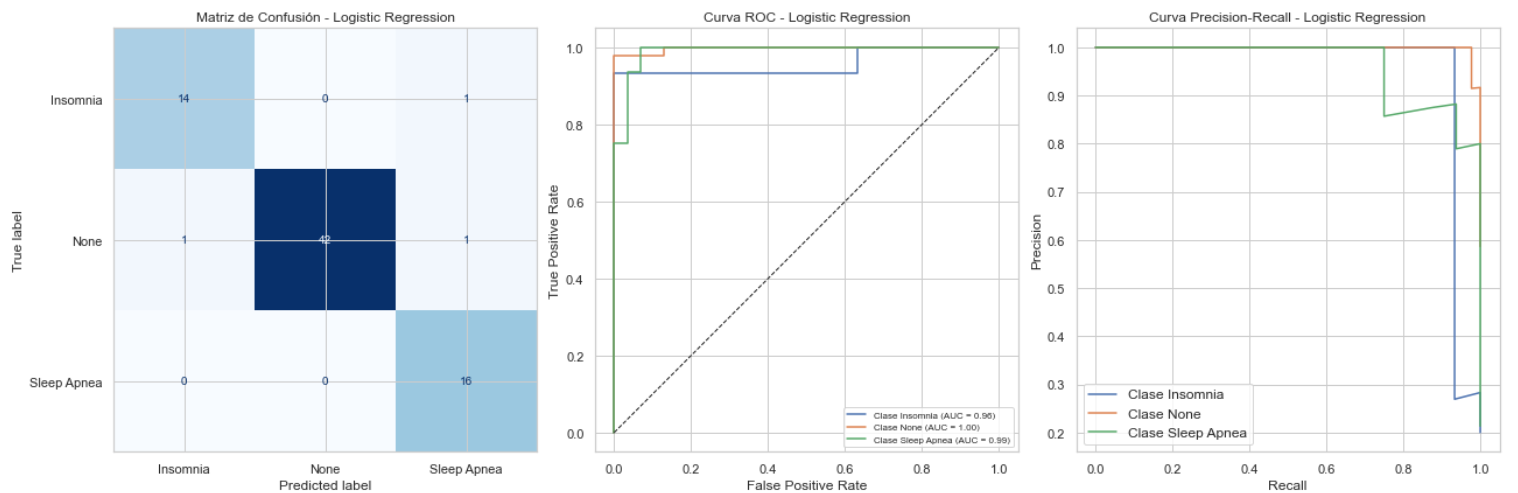
\includegraphics[width=\textwidth]{img/curvas_LR.png}
    \caption{Evaluación visual del modelo \textit{Logistic Regression}: matriz de confusión, curva ROC-AUC y Precision-Recall.}
    \label{fig:curvas_lr}
\end{figure}

\subsubsection{Comparación de curvas ROC-AUC por clase}

A continuación se muestran las curvas ROC-AUC de los cinco modelos, diferenciadas por clase. Esta representación permite observar con mayor detalle el rendimiento discriminativo para cada tipo de trastorno del sueño. 

\begin{figure}[H]
    \centering
    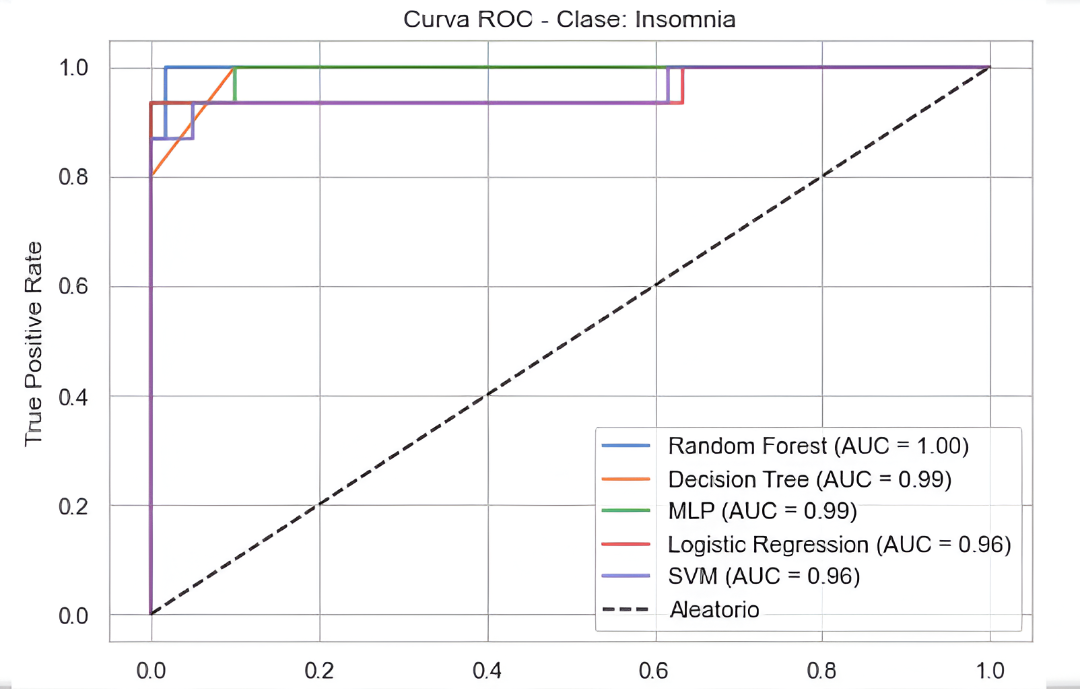
\includegraphics[width=0.9\textwidth]{img/roc_insomnia.png}
    \caption{Curva ROC-AUC para la clase \texttt{Insomnia}.}
    \label{fig:roc_insomnia}
\end{figure}

\begin{figure}[H]
    \centering
    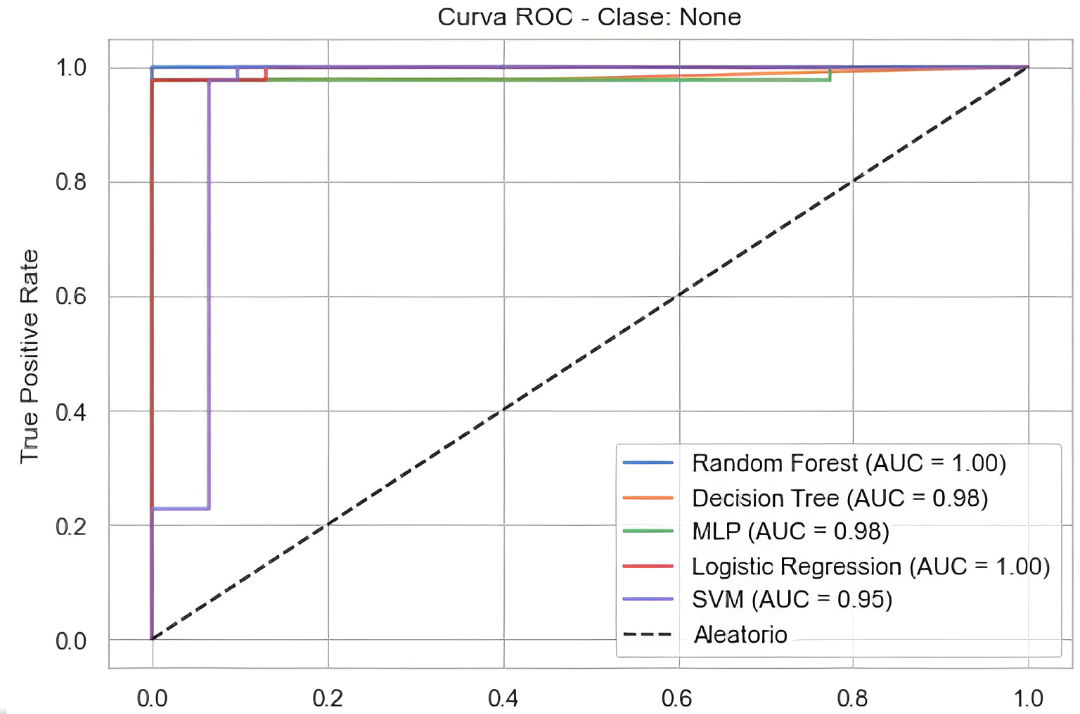
\includegraphics[width=0.9\textwidth]{img/roc_none.png}
    \caption{Curva ROC-AUC para la clase \texttt{None}.}
    \label{fig:roc_none}
\end{figure}

\begin{figure}[H]
    \centering
    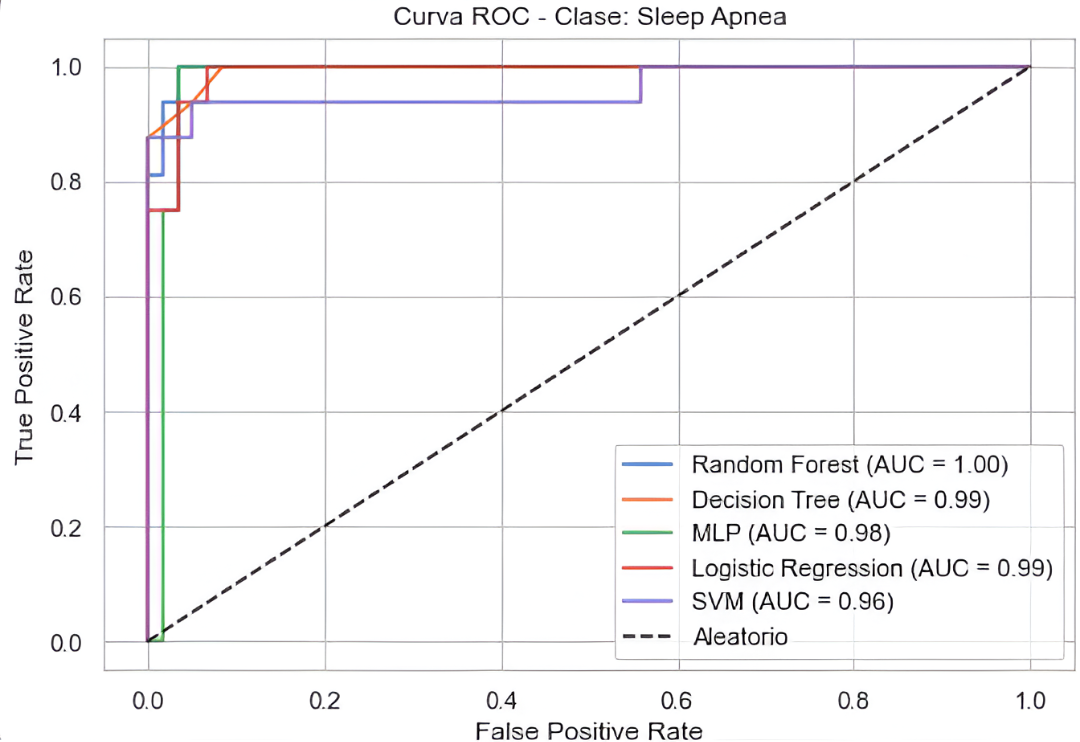
\includegraphics[width=0.8\textwidth]{img/roc_apnea.png}
    \caption{Curva ROC-AUC para la clase \texttt{Sleep Apnea}.}
    \label{fig:roc_apnea}
\end{figure}

Se observa que los modelos \textit{Random Forest} y \textit{MLP} mantienen una capacidad discriminativa sobresaliente en todas las clases, con áreas bajo la curva (AUC) superiores al 0.98. Este comportamiento se mantiene especialmente estable en la clase \texttt{Sleep Apnea}, lo que resulta crítico desde un punto de vista clínico, ya que permite minimizar los falsos negativos en una condición potencialmente grave.

El modelo \textit{Logistic Regression} también muestra un desempeño competitivo, alcanzando un AUC de 1.00 en la clase \texttt{None} y de 0.96 en \texttt{Insomnia} y \texttt{Sleep Apnea}, lo cual refleja su equilibrio entre precisión y sensibilidad.

Por su parte, el modelo \textit{SVM} presenta una ligera caída en el AUC en todas las clases (entre 0.95 y 0.96), aunque aún dentro de un margen aceptable. \textit{Decision Tree} tiene un rendimiento intermedio, con AUC de 0.98--0.99, pero con una curva más irregular.

Estas diferencias sugieren que, aunque todos los modelos son razonablemente fiables, \textit{Random Forest} y \textit{MLP} ofrecen mayor robustez en situaciones clínicas reales donde la correcta discriminación entre clases es fundamental.

\vspace{1em}

\subsubsection{Comparación de curvas Precision-Recall por clase}

A continuación se presentan las curvas Precision-Recall, especialmente relevantes en contextos con clases desbalanceadas. Estas permiten evaluar la capacidad del modelo para mantener una alta precisión a medida que se incrementa la sensibilidad.


\begin{figure}[H]
    \centering
    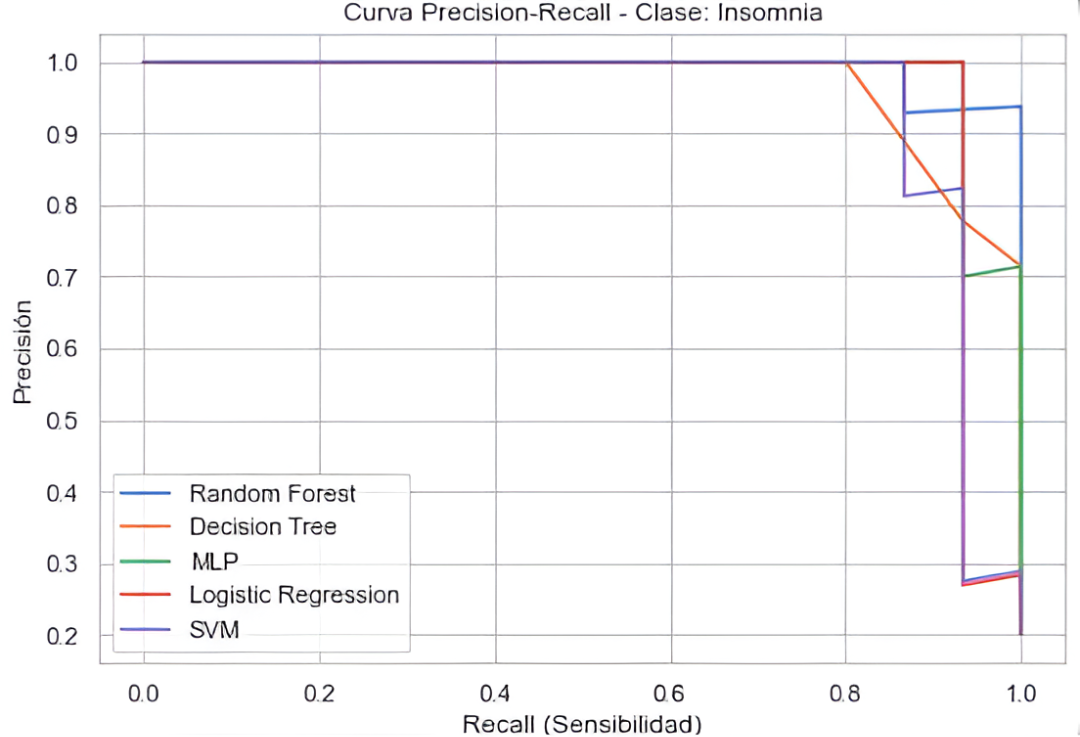
\includegraphics[width=0.8\textwidth]{img/pr_insomnia.png}
    \caption{Curva Precision-Recall para la clase \texttt{Insomnia}.}
    \label{fig:pr_insomnia}
\end{figure}

\begin{figure}[H]
    \centering
    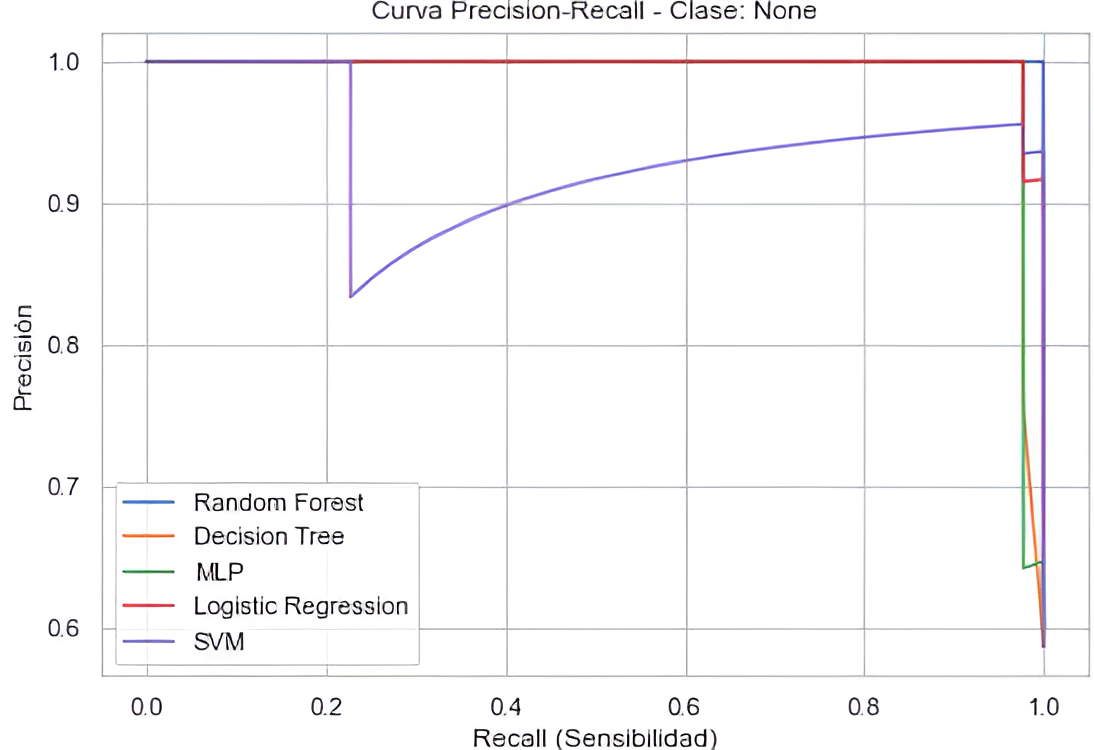
\includegraphics[width=0.8\textwidth]{img/pr_none.png}
    \caption{Curva Precision-Recall para la clase \texttt{None}.}
    \label{fig:pr_none}
\end{figure}

\begin{figure}[H]
    \centering
    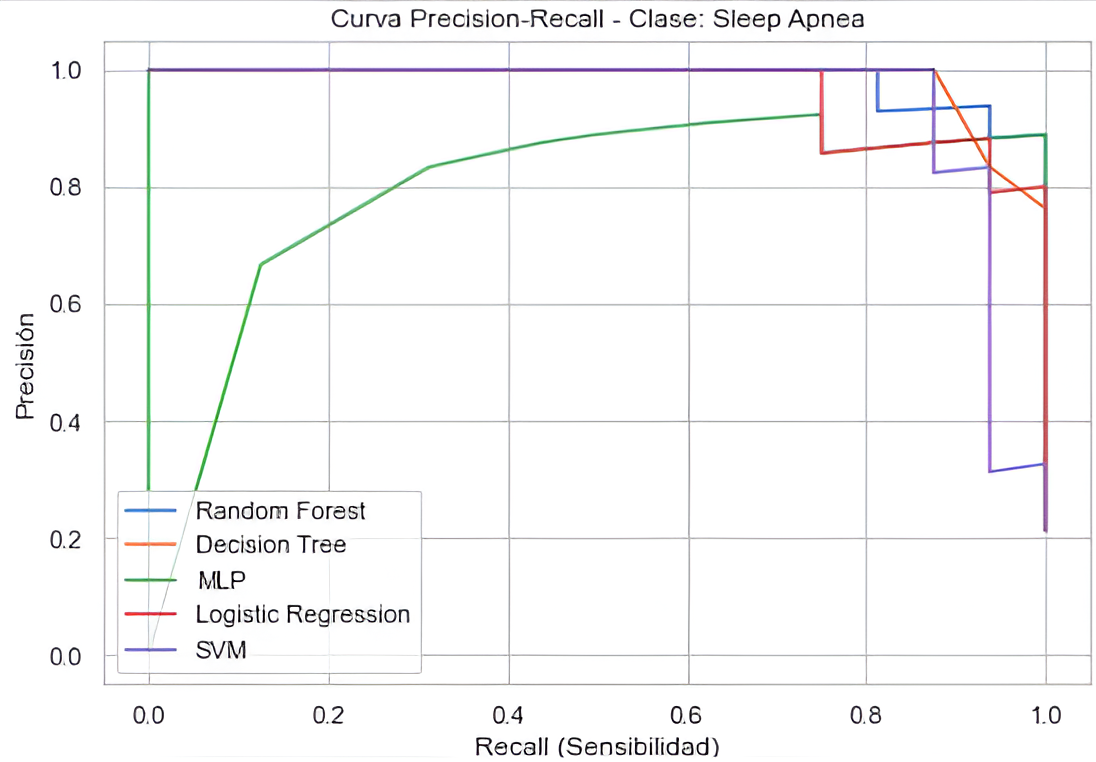
\includegraphics[width=0.8\textwidth]{img/pr_apnea.png}
    \caption{Curva Precision-Recall para la clase \texttt{Sleep Apnea}.}
    \label{fig:pr_apnea}
\end{figure}

En cuanto a las curvas Precision-Recall, se reafirma el buen comportamiento de \textit{Random Forest} y \textit{MLP}, especialmente en las clases minoritarias. En \texttt{Sleep Apnea}, \textit{Random Forest} mantiene una alta precisión incluso con niveles elevados de recall, lo que indica que logra identificar a la mayoría de los casos positivos sin generar un exceso de falsos positivos.

\textit{MLP}, por su parte, destaca en la clase \texttt{Insomnia}, mostrando una curva más estable y cercana al óptimo. Esto refuerza su idoneidad en entornos clínicos donde la sensibilidad debe ser prioritaria.

En contraste, modelos como \textit{SVM} y \textit{Decision Tree} presentan curvas más irregulares y una caída más abrupta de la precisión a medida que aumenta el recall, lo cual podría comprometer su fiabilidad en un sistema de cribado automatizado.

Estas curvas confirman que no solo es importante qué clase se predice, sino también con qué confianza lo hace el modelo, un aspecto clave cuando se trata de emitir alertas médicas.


\subsubsection{Resumen conjunto de desempeño por clase}

El análisis gráfico detallado permite identificar patrones diferenciales en el comportamiento de los modelos por clase. En la clase \texttt{Insomnia}, los modelos Random Forest y MLP ofrecen curvas ROC-AUC y Precision-Recall elevadas y estables, lo que sugiere una buena capacidad para detectar esta condición con alta sensibilidad sin comprometer la precisión. En cambio, modelos como SVM o Decision Tree muestran ligeros descensos en la precisión, indicando mayor tendencia a generar falsos positivos.

\begin{table}[H]
\centering
\small
\begin{tabular}{lccc|ccc}
\toprule
\multirow{2}{*}{\textbf{Modelo}} & \multicolumn{3}{c|}{\textbf{AUC-ROC}} & \multicolumn{3}{c}{\textbf{AUC-PR}} \\
& \textbf{Insomnia} & \textbf{None} & \textbf{Apnea} & \textbf{Insomnia} & \textbf{None} & \textbf{Apnea} \\
\midrule
Random Forest       & 1.00 & 1.00 & 1.00 & 0.94 & 0.99 & 0.96 \\
MLP                 & 0.99 & 0.98 & 0.98 & 0.87 & 0.98 & 0.93 \\
Logistic Regression & 0.96 & 1.00 & 0.99 & 0.93 & 1.00 & 0.91 \\
Decision Tree       & 0.99 & 0.98 & 0.99 & 0.89 & 0.99 & 0.88 \\
SVM                 & 0.96 & 0.95 & 0.96 & 0.91 & 0.94 & 0.87 \\
\bottomrule
\end{tabular}
\caption{Comparativa de AUC-ROC y AUC-PR por clase en los cinco modelos evaluados.}
\label{tab:auc-por-clase}
\end{table}

La Tabla~\ref{tab:auc-por-clase} refuerza este análisis al mostrar los valores medios de las métricas AUC-ROC y AUC-PR para cada clase. Se confirma que Random Forest y MLP alcanzan los mejores resultados en la clase \texttt{Insomnia}, destacando en ambas métricas sobre el resto.

Para la clase \texttt{None}, todos los modelos alcanzan valores muy altos de AUC y precisión, lo que es esperable dado que se trata de la clase mayoritaria y, por tanto, más representada durante el entrenamiento. Esto refuerza la necesidad de priorizar el análisis específico en las clases clínicas más relevantes.

En el caso de \texttt{Sleep Apnea}, la curva Precision-Recall de MLP destaca por mantener un recall próximo al 1.0, aunque con menor precisión en ciertos rangos de umbral. Random Forest, en cambio, presenta un mayor equilibrio entre ambas métricas, siendo capaz de identificar correctamente la mayoría de los casos sin aumentar el número de falsos positivos de forma excesiva. Esto lo convierte en un candidato sólido para su implementación en la herramienta final, donde el balance clínico entre sensibilidad y especificidad es crucial.

En conjunto, la descomposición por clase de estas curvas ofrece una perspectiva rica y más precisa que las métricas globales, reforzando la validez del análisis multiclase en un contexto sanitario.


\subsection{Comparación final y selección del modelo óptimo}

Tras analizar las métricas cuantitativas y los resultados gráficos, se seleccionaron dos modelos como los más prometedores durante la fase experimental: \textbf{Random Forest} y \textbf{MLP}. Ambos presentaron un rendimiento sobresaliente en las métricas evaluadas —\textit{accuracy}, \textit{F1-score macro}, \textit{recall} y \textit{precisión}—, así como una excelente capacidad discriminativa entre clases.

La elección se basó tanto en los valores obtenidos como en las curvas ROC-AUC y Precision-Recall, que confirmaron un comportamiento consistente y fiable. Ambos modelos compartían las siguientes características clave:


\begin{itemize}
    \item Área bajo la curva (AUC) superior a 0.95 en todas las clases.
    \item Buen equilibrio entre precisión y sensibilidad, especialmente en \texttt{Sleep Apnea}.
    \item Estabilidad en distintas particiones del conjunto de validación.
\end{itemize}

\textbf{Random Forest} destacó por su mayor interpretabilidad y precisión en la clase \texttt{Sleep Apnea}, lo que facilita su trazabilidad en entornos clínicos. Por su parte, \textbf{MLP} alcanzó un \textit{recall} perfecto en esa misma clase, lo que resulta ventajoso en contextos donde se prioriza la sensibilidad diagnóstica para minimizar falsos negativos.


Ambos modelos fueron evaluados como candidatos finales, pero finalmente se seleccionó Random Forest para su integración definitiva en la aplicación por su capacidad explicativa. Este modelo fue calibrado mediante \texttt{CalibratedClassifierCV} y guardado en el archivo:

\begin{itemize}
  \item \texttt{random\_forest\_model.joblib}
\end{itemize}

La validación práctica y externa de este modelo, incluyendo su evaluación con datos del dispositivo O2Ring, se detalla en la siguiente sección.


\subsection{Evaluación comparativa con y sin la variable \texttt{Occupation}}

Con el objetivo de evaluar el impacto real de la variable \texttt{Occupation} en la capacidad predictiva del modelo, se construyó una versión alternativa del sistema eliminando dicha característica del conjunto de entrenamiento. Esta modificación tenía como objetivo analizar si la ocupación laboral estaba introduciendo un sesgo en las predicciones, y si el modelo era capaz de mantener un rendimiento clínico aceptable sin dicha información. Cabe señalar que algunas ocupaciones estaban sobrerrepresentadas en ciertas clases del conjunto de entrenamiento, lo que podría inducir al modelo a establecer falsas asociaciones.

Para garantizar un análisis controlado, se mantuvieron constantes todas las demás variables, de forma que cualquier cambio en la predicción pudiera atribuirse exclusivamente a la presencia o ausencia de la variable \texttt{Occupation}. La validación se realizó sobre tres perfiles clínicos reales representativos: un paciente con apnea del sueño (A), un sujeto sano (B) y un paciente con insomnio leve (C). Las predicciones se compararon entre ambas versiones del modelo, manteniendo los parámetros fisiológicos constantes (edad, sexo, IMC) y ajustando únicamente variables como pasos diarios, duración del sueño o nivel de estrés para reforzar la coherencia clínica.

\begin{table}[H]
\centering
\begin{tabular}{|c|c|c|c|c|}
\hline
\textbf{Paciente} & \textbf{Diagnóst esperado} & \textbf{Con Occupation} & \textbf{Sin Occupation} \\
\hline
A (Apnea)   & Apnea del sueño     & Sleep Apnea (70.0\%) & Insomnia (59.0\%) \\
B (Sano)    & Ninguno             & Sleep Apnea (59.0\%) & None (98.0\%) \\
C (Insomnio) & Insomnio subjetivo & Sleep Apnea (58.0\%) & Insomnia (67.0\%) \\
\hline
\end{tabular}
\caption{Comparativa de predicciones entre ambas versiones del modelo usando los perfiles clínicos reales.}
\end{table}


Los resultados revelan un patrón claro: la versión \textbf{con la variable \texttt{Occupation}} tiende a \textbf{sobrediagnosticar apnea del sueño} en todos los casos, incluso cuando no hay evidencia clínica suficiente, como ocurre con los pacientes B y C. Esta tendencia sugiere un sobreajuste del modelo o un sesgo inducido por la ocupación laboral.

Por el contrario, la versión \textbf{sin \texttt{Occupation}} mostró un comportamiento más prudente y clínicamente coherente. Fue capaz de clasificar correctamente al paciente sano y de aproximarse mejor a la predicción esperada en el caso de insomnio, aunque aún presenta margen de mejora en sensibilidad. Este comportamiento indica que, si bien la variable \texttt{Occupation} aporta poder predictivo, también introduce un riesgo clínico si no se maneja cuidadosamente.

En consecuencia, se optó por mantener el modelo con \texttt{Occupation} calibrado como núcleo del sistema desplegado, dada su estabilidad, calibración previa y compatibilidad con las herramientas de interpretabilidad. No obstante, se incorporaron advertencias explícitas en la interfaz sobre el carácter orientativo del sistema y la posible influencia de variables contextuales. Esta evaluación pone de manifiesto la importancia de revisar críticamente el uso de variables categóricas con fuerte carga contextual y de diseñar mecanismos de mitigación de sesgos en futuros desarrollos clínicos.


\section{Validación externa con datos reales del dispositivo O2Ring}

Con el objetivo de evaluar la capacidad del modelo para generalizar fuera del conjunto de entrenamiento, se realizó una validación externa utilizando datos fisiológicos recogidos con el pulsioxímetro comercial O2Ring. Esta prueba permite estimar el rendimiento del sistema en condiciones clínicas reales.

Se seleccionaron tres pacientes reales con perfiles representativos de las tres clases objetivo del problema: apnea del sueño, individuo sano e insomnio leve. A continuación se resume su análisis individual.


\subsection{Paciente A – Apnea del sueño}

\begin{itemize}
    \item Edad: 57 años, IMC: 31.8 (obesidad)
    \item Duración del sueño: 5h 53min
    \item Saturación media: 89\%, mínima: 70\%
    \item Tiempo con SpO\textsubscript{2} < 90\%: 3h 17min
    \item ODI 3\%: 43.3/h
    \item FC media: 61 bpm
\end{itemize}

\textbf{Diagnóstico clínico esperado:} Apnea moderada-grave.
\textbf{Predicción del modelo:} Sleep Apnea (70.4\%).  
\textbf{¿Acertó?} Sí.

\subsection{Paciente B – Perfil sano}

\begin{itemize}
    \item Edad: 32 años, IMC: 20.6 (peso normal)
    \item Duración del sueño: 8h 28min
    \item Saturación media: 96\%, mínima: 92\%
    \item ODI 3\%: 0.1/h, SpO\textsubscript{2} < 90\%: 0s
    \item FC media: 51 bpm
\end{itemize}

\textbf{Diagnóstico clínico esperado:} Sin trastornos.  
\textbf{Predicción del modelo:} Sleep Apnea (56.0\%).  
\textbf{¿Acertó?} No (falso positivo).

\subsection{Paciente C – Perfil compatible con insomnio}

\begin{itemize}
    \item Edad: 55 años, IMC: 25.4 (límite sobrepeso)
    \item Duración del sueño: 7h, calidad: 4/10
    \item Estrés alto, 1 día de deporte semanal, 5000 pasos diarios
    \item Presión arterial: 120/75, FC: 48 bpm
\end{itemize}

\textbf{Diagnóstico clínico esperado:} Insomnio leve subjetivo.  
\textbf{Predicción del modelo:} Sleep Apnea (72.7\%).  
\textbf{¿Acertó?} No (falso positivo).


\subsection{Resumen de resultados}

\begin{table}[H]
\centering
\begin{tabular}{|c|c|c|c|c|}
\hline
\textbf{Paciente} & \textbf{Diagnóstico esperado} & \textbf{Predicción} & \textbf{¿Acertó?} \\
\hline
A & Apnea del sueño & Sleep Apnea (70.4\%) & Sí \\
B & Ninguno         & Sleep Apnea (60.0\%) & No \\
C & Insomnio        & Sleep Apnea (72.7\%) & No \\
\hline
\end{tabular}
\caption{Validación externa con datos reales recogidos mediante O2Ring.}
\end{table}


Los resultados de esta validación externa revelan limitaciones importantes del sistema desplegado. Aunque en el caso A se acertó el diagnóstico con alta probabilidad, los casos B y C fueron clasificados erróneamente como apnea del sueño, a pesar de que sus métricas fisiológicas no justificaban dicho diagnóstico.

Estos errores confirman que el modelo, entrenado exclusivamente con variables demográficas y de estilo de vida, carece de sensibilidad suficiente para distinguir correctamente entre insomnio, sujetos sanos y apnea real. La ausencia de variables biométricas clave como SpO$_2$ nocturna, ODI o eventos respiratorios limita la capacidad clínica del sistema para ofrecer diagnósticos fiables.

Este análisis pone de manifiesto la necesidad de incorporar señales fisiológicas reales en futuras versiones del modelo, así como de realizar entrenamientos con conjuntos de datos validados clínicamente. Solo así será posible desarrollar sistemas de ayuda al diagnóstico que sean realmente útiles y seguros en entornos reales.

\section{Discusión}

Este trabajo ha demostrado la viabilidad de desarrollar un sistema predictivo funcional para la detección automática de trastornos del sueño, empleando exclusivamente datos clínicos y de estilo de vida. La implementación completa del pipeline —desde la preparación de datos hasta la validación externa y la integración en una aplicación web— permite reflexionar sobre la utilidad real de este tipo de herramientas, sus limitaciones actuales y sus implicaciones futuras.


\subsection{Importancia de las métricas en el contexto clínico}

En un entorno sanitario, no todas las métricas de evaluación tienen el mismo peso. Aunque el \textit{accuracy} proporciona una visión general del rendimiento del modelo, puede resultar engañosa en problemas con clases desbalanceadas o consecuencias clínicas asimétricas.

En este estudio, se priorizó el \textbf{recall} en la clase \texttt{Sleep Apnea}, dado que no detectar un caso real puede tener consecuencias graves para el paciente. Por ello, este indicador se consideró crítico en todas las fases de evaluación y selección del modelo, especialmente al comparar candidatos como \textit{Random Forest} y \textit{MLP}.


\subsection{Errores comunes y clases más conflictivas}

Durante las validaciones, tanto internas como externas, se observó que la clase \texttt{Sleep Apnea} concentraba la mayoría de los errores, especialmente en forma de falsos positivos. El sistema tendía a sobrediagnosticar esta clase en perfiles donde no existía evidencia clínica suficiente, como ocurrió con los pacientes B y C durante la validación externa.

En contraste, la clase \texttt{Insomnia} fue identificada con mayor estabilidad en varios modelos, lo que sugiere que sus rasgos subjetivos (calidad del sueño, duración baja, estrés elevado) estaban mejor representados en los datos y eran más fáciles de distinguir estadísticamente.



\subsection{Limitaciones del sistema y del conjunto de datos}

Las principales limitaciones que condicionan el rendimiento clínico del sistema son:

\begin{itemize}
    \item \textbf{Tamaño reducido del dataset}: solo 374 registros, lo que limita la generalización del modelo a poblaciones reales más diversas.
    \item \textbf{Datos autodeclarados}: variables como la calidad del sueño, el nivel de estrés o la duración del sueño están basadas en percepciones subjetivas del paciente, introduciendo sesgos de respuesta.
    \item \textbf{Desequilibrio de clases}: la clase \texttt{None} representa más del 50\% del total, lo que afecta a la estabilidad del aprendizaje y puede favorecer predicciones triviales.
    \item \textbf{Ausencia de datos fisiológicos reales}: el modelo no conoce variables clave como SpO$_2$, ODI, eventos respiratorios o movimiento nocturno, lo que limita su valor clínico.
\end{itemize}

Aunque se evaluaron técnicas de balanceo como SMOTE, sus efectos no fueron consistentes, y en algunos casos derivaron en sobreajuste. Se optó por enfoques más conservadores como el ajuste de pesos de clase y la calibración probabilística.

\subsection{Impacto de la variable \texttt{Occupation}}

Uno de los hallazgos más relevantes del estudio fue el impacto de la variable \texttt{Occupation} en las predicciones. El modelo entrenado con esta variable mostró un sesgo claro hacia la clase \texttt{Sleep Apnea}, clasificando erróneamente perfiles sanos o compatibles con insomnio como casos de apnea, incluso tras modificar otras variables.

La comparación con una versión del modelo sin \texttt{Occupation} reveló un comportamiento más prudente y alineado con el diagnóstico esperado en varios casos. Sin embargo, este modelo alternativo no fue integrado en la aplicación final, ya que no estaba calibrado ni preparado para su despliegue. Aun así, la existencia de este sesgo justifica plenamente la incorporación de advertencias explícitas en la app y refuerza la necesidad de revisar críticamente el uso de variables socioeconómicas en contextos clínicos.


\subsection{Relación con la literatura}

Los resultados obtenidos son coherentes con estudios previos que emplean modelos de machine learning para el cribado de trastornos del sueño a partir de datos tabulados. El trabajo de \textit{Alnour et al. (2024)}\footnote{\cite{alnour2024kaggle}}, base del dataset utilizado, ya demostraba que modelos como \textit{Random Forest} o \textit{SVM} ofrecían buen rendimiento en tareas de clasificación, aunque sin explorar su integración práctica.

Este proyecto ha ido un paso más allá al incluir explicabilidad mediante SHAP, validación con pacientes reales monitorizados con O2Ring, y la implementación completa de una aplicación web interactiva y descargable.


\subsection{Implicaciones y proyección}

A pesar de sus limitaciones, el sistema propuesto presenta potencial como herramienta de cribado preliminar o de concienciación en contextos sin acceso a polisomnografía ni actigrafía. Su facilidad de uso, la interpretabilidad integrada y la generación automática de informes podrían facilitar su adopción en entornos comunitarios o de atención primaria.

Sin embargo, la validación con pacientes reales ha puesto de manifiesto que la fiabilidad clínica del modelo es limitada si no se integran variables fisiológicas reales. En este sentido, se propone como línea futura la recogida de datos multimodales —incluyendo señales del sueño, pulsioximetría y movimiento— que permitan entrenar modelos más precisos y clínicamente útiles.

Los siguientes capítulos recogen las conclusiones generales del trabajo y propuestas concretas para su mejora.